% Options for packages loaded elsewhere
\PassOptionsToPackage{unicode}{hyperref}
\PassOptionsToPackage{hyphens}{url}
\PassOptionsToPackage{dvipsnames,svgnames,x11names}{xcolor}
%
\documentclass[
  letterpaper,
  DIV=11,
  numbers=noendperiod]{scrartcl}

\usepackage{amsmath,amssymb}
\usepackage{iftex}
\ifPDFTeX
  \usepackage[T1]{fontenc}
  \usepackage[utf8]{inputenc}
  \usepackage{textcomp} % provide euro and other symbols
\else % if luatex or xetex
  \usepackage{unicode-math}
  \defaultfontfeatures{Scale=MatchLowercase}
  \defaultfontfeatures[\rmfamily]{Ligatures=TeX,Scale=1}
\fi
\usepackage{lmodern}
\ifPDFTeX\else  
    % xetex/luatex font selection
\fi
% Use upquote if available, for straight quotes in verbatim environments
\IfFileExists{upquote.sty}{\usepackage{upquote}}{}
\IfFileExists{microtype.sty}{% use microtype if available
  \usepackage[]{microtype}
  \UseMicrotypeSet[protrusion]{basicmath} % disable protrusion for tt fonts
}{}
\makeatletter
\@ifundefined{KOMAClassName}{% if non-KOMA class
  \IfFileExists{parskip.sty}{%
    \usepackage{parskip}
  }{% else
    \setlength{\parindent}{0pt}
    \setlength{\parskip}{6pt plus 2pt minus 1pt}}
}{% if KOMA class
  \KOMAoptions{parskip=half}}
\makeatother
\usepackage{xcolor}
\setlength{\emergencystretch}{3em} % prevent overfull lines
\setcounter{secnumdepth}{-\maxdimen} % remove section numbering
% Make \paragraph and \subparagraph free-standing
\makeatletter
\ifx\paragraph\undefined\else
  \let\oldparagraph\paragraph
  \renewcommand{\paragraph}{
    \@ifstar
      \xxxParagraphStar
      \xxxParagraphNoStar
  }
  \newcommand{\xxxParagraphStar}[1]{\oldparagraph*{#1}\mbox{}}
  \newcommand{\xxxParagraphNoStar}[1]{\oldparagraph{#1}\mbox{}}
\fi
\ifx\subparagraph\undefined\else
  \let\oldsubparagraph\subparagraph
  \renewcommand{\subparagraph}{
    \@ifstar
      \xxxSubParagraphStar
      \xxxSubParagraphNoStar
  }
  \newcommand{\xxxSubParagraphStar}[1]{\oldsubparagraph*{#1}\mbox{}}
  \newcommand{\xxxSubParagraphNoStar}[1]{\oldsubparagraph{#1}\mbox{}}
\fi
\makeatother

\usepackage{color}
\usepackage{fancyvrb}
\newcommand{\VerbBar}{|}
\newcommand{\VERB}{\Verb[commandchars=\\\{\}]}
\DefineVerbatimEnvironment{Highlighting}{Verbatim}{commandchars=\\\{\}}
% Add ',fontsize=\small' for more characters per line
\usepackage{framed}
\definecolor{shadecolor}{RGB}{241,243,245}
\newenvironment{Shaded}{\begin{snugshade}}{\end{snugshade}}
\newcommand{\AlertTok}[1]{\textcolor[rgb]{0.68,0.00,0.00}{#1}}
\newcommand{\AnnotationTok}[1]{\textcolor[rgb]{0.37,0.37,0.37}{#1}}
\newcommand{\AttributeTok}[1]{\textcolor[rgb]{0.40,0.45,0.13}{#1}}
\newcommand{\BaseNTok}[1]{\textcolor[rgb]{0.68,0.00,0.00}{#1}}
\newcommand{\BuiltInTok}[1]{\textcolor[rgb]{0.00,0.23,0.31}{#1}}
\newcommand{\CharTok}[1]{\textcolor[rgb]{0.13,0.47,0.30}{#1}}
\newcommand{\CommentTok}[1]{\textcolor[rgb]{0.37,0.37,0.37}{#1}}
\newcommand{\CommentVarTok}[1]{\textcolor[rgb]{0.37,0.37,0.37}{\textit{#1}}}
\newcommand{\ConstantTok}[1]{\textcolor[rgb]{0.56,0.35,0.01}{#1}}
\newcommand{\ControlFlowTok}[1]{\textcolor[rgb]{0.00,0.23,0.31}{\textbf{#1}}}
\newcommand{\DataTypeTok}[1]{\textcolor[rgb]{0.68,0.00,0.00}{#1}}
\newcommand{\DecValTok}[1]{\textcolor[rgb]{0.68,0.00,0.00}{#1}}
\newcommand{\DocumentationTok}[1]{\textcolor[rgb]{0.37,0.37,0.37}{\textit{#1}}}
\newcommand{\ErrorTok}[1]{\textcolor[rgb]{0.68,0.00,0.00}{#1}}
\newcommand{\ExtensionTok}[1]{\textcolor[rgb]{0.00,0.23,0.31}{#1}}
\newcommand{\FloatTok}[1]{\textcolor[rgb]{0.68,0.00,0.00}{#1}}
\newcommand{\FunctionTok}[1]{\textcolor[rgb]{0.28,0.35,0.67}{#1}}
\newcommand{\ImportTok}[1]{\textcolor[rgb]{0.00,0.46,0.62}{#1}}
\newcommand{\InformationTok}[1]{\textcolor[rgb]{0.37,0.37,0.37}{#1}}
\newcommand{\KeywordTok}[1]{\textcolor[rgb]{0.00,0.23,0.31}{\textbf{#1}}}
\newcommand{\NormalTok}[1]{\textcolor[rgb]{0.00,0.23,0.31}{#1}}
\newcommand{\OperatorTok}[1]{\textcolor[rgb]{0.37,0.37,0.37}{#1}}
\newcommand{\OtherTok}[1]{\textcolor[rgb]{0.00,0.23,0.31}{#1}}
\newcommand{\PreprocessorTok}[1]{\textcolor[rgb]{0.68,0.00,0.00}{#1}}
\newcommand{\RegionMarkerTok}[1]{\textcolor[rgb]{0.00,0.23,0.31}{#1}}
\newcommand{\SpecialCharTok}[1]{\textcolor[rgb]{0.37,0.37,0.37}{#1}}
\newcommand{\SpecialStringTok}[1]{\textcolor[rgb]{0.13,0.47,0.30}{#1}}
\newcommand{\StringTok}[1]{\textcolor[rgb]{0.13,0.47,0.30}{#1}}
\newcommand{\VariableTok}[1]{\textcolor[rgb]{0.07,0.07,0.07}{#1}}
\newcommand{\VerbatimStringTok}[1]{\textcolor[rgb]{0.13,0.47,0.30}{#1}}
\newcommand{\WarningTok}[1]{\textcolor[rgb]{0.37,0.37,0.37}{\textit{#1}}}

\providecommand{\tightlist}{%
  \setlength{\itemsep}{0pt}\setlength{\parskip}{0pt}}\usepackage{longtable,booktabs,array}
\usepackage{calc} % for calculating minipage widths
% Correct order of tables after \paragraph or \subparagraph
\usepackage{etoolbox}
\makeatletter
\patchcmd\longtable{\par}{\if@noskipsec\mbox{}\fi\par}{}{}
\makeatother
% Allow footnotes in longtable head/foot
\IfFileExists{footnotehyper.sty}{\usepackage{footnotehyper}}{\usepackage{footnote}}
\makesavenoteenv{longtable}
\usepackage{graphicx}
\makeatletter
\newsavebox\pandoc@box
\newcommand*\pandocbounded[1]{% scales image to fit in text height/width
  \sbox\pandoc@box{#1}%
  \Gscale@div\@tempa{\textheight}{\dimexpr\ht\pandoc@box+\dp\pandoc@box\relax}%
  \Gscale@div\@tempb{\linewidth}{\wd\pandoc@box}%
  \ifdim\@tempb\p@<\@tempa\p@\let\@tempa\@tempb\fi% select the smaller of both
  \ifdim\@tempa\p@<\p@\scalebox{\@tempa}{\usebox\pandoc@box}%
  \else\usebox{\pandoc@box}%
  \fi%
}
% Set default figure placement to htbp
\def\fps@figure{htbp}
\makeatother

\usepackage{booktabs}
\usepackage{caption}
\usepackage{longtable}
\usepackage{colortbl}
\usepackage{array}
\usepackage{anyfontsize}
\usepackage{multirow}
\KOMAoption{captions}{tableheading}
\makeatletter
\@ifpackageloaded{caption}{}{\usepackage{caption}}
\AtBeginDocument{%
\ifdefined\contentsname
  \renewcommand*\contentsname{Table of contents}
\else
  \newcommand\contentsname{Table of contents}
\fi
\ifdefined\listfigurename
  \renewcommand*\listfigurename{List of Figures}
\else
  \newcommand\listfigurename{List of Figures}
\fi
\ifdefined\listtablename
  \renewcommand*\listtablename{List of Tables}
\else
  \newcommand\listtablename{List of Tables}
\fi
\ifdefined\figurename
  \renewcommand*\figurename{Figure}
\else
  \newcommand\figurename{Figure}
\fi
\ifdefined\tablename
  \renewcommand*\tablename{Table}
\else
  \newcommand\tablename{Table}
\fi
}
\@ifpackageloaded{float}{}{\usepackage{float}}
\floatstyle{ruled}
\@ifundefined{c@chapter}{\newfloat{codelisting}{h}{lop}}{\newfloat{codelisting}{h}{lop}[chapter]}
\floatname{codelisting}{Listing}
\newcommand*\listoflistings{\listof{codelisting}{List of Listings}}
\makeatother
\makeatletter
\makeatother
\makeatletter
\@ifpackageloaded{caption}{}{\usepackage{caption}}
\@ifpackageloaded{subcaption}{}{\usepackage{subcaption}}
\makeatother

\usepackage{bookmark}

\IfFileExists{xurl.sty}{\usepackage{xurl}}{} % add URL line breaks if available
\urlstyle{same} % disable monospaced font for URLs
\hypersetup{
  pdftitle={Homework Assignment 2},
  pdfauthor={Ixel},
  colorlinks=true,
  linkcolor={blue},
  filecolor={Maroon},
  citecolor={Blue},
  urlcolor={Blue},
  pdfcreator={LaTeX via pandoc}}


\title{Homework Assignment 2}
\author{Ixel}
\date{2025-10-19}

\begin{document}
\maketitle


\subsection{Exploring patterns of environmental
justice}\label{exploring-patterns-of-environmental-justice}

\paragraph{Set Up}\label{set-up}

\begin{Shaded}
\begin{Highlighting}[]
\CommentTok{\# Librarys used to complete this homework}

\FunctionTok{library}\NormalTok{(sf) }\CommentTok{\# for vector data }
\FunctionTok{library}\NormalTok{(tmap) }\CommentTok{\# for static and interactive maps}
\FunctionTok{library}\NormalTok{(here)}
\FunctionTok{library}\NormalTok{(spData) }
\FunctionTok{library}\NormalTok{(tidyverse)}
\FunctionTok{library}\NormalTok{(dplyr)}
\FunctionTok{library}\NormalTok{(gt)}
\FunctionTok{library}\NormalTok{(viridis)}
\end{Highlighting}
\end{Shaded}

\begin{Shaded}
\begin{Highlighting}[]
\CommentTok{\# Spatial data object to plot}

\CommentTok{\# EJScreen }
\NormalTok{ejscreen }\OtherTok{\textless{}{-}} \FunctionTok{st\_read}\NormalTok{(}\FunctionTok{here}\NormalTok{(}\StringTok{"data/ejscreen/EJSCREEN\_2023\_BG\_StatePct\_with\_AS\_CNMI\_GU\_VI.gdb"}\NormalTok{))}
\end{Highlighting}
\end{Shaded}

\begin{verbatim}
Reading layer `EJSCREEN_StatePctiles_with_AS_CNMI_GU_VI' from data source 
  `C:\Users\Donaji\Documents\MEDS\EDS-223\HomeWork\EDS223-HW2\data\ejscreen\EJSCREEN_2023_BG_StatePct_with_AS_CNMI_GU_VI.gdb' 
  using driver `OpenFileGDB'
Simple feature collection with 243021 features and 223 fields
Geometry type: MULTIPOLYGON
Dimension:     XY
Bounding box:  xmin: -19951910 ymin: -1617130 xmax: 16259830 ymax: 11554350
Projected CRS: WGS 84 / Pseudo-Mercator
\end{verbatim}

\begin{Shaded}
\begin{Highlighting}[]
\CommentTok{\# HOLC Redlining}
\NormalTok{ holc }\OtherTok{\textless{}{-}} \FunctionTok{st\_read}\NormalTok{(}\FunctionTok{here}\NormalTok{(}\StringTok{"data/mapping{-}inequality/mapping{-}inequality{-}los{-}angeles.json"}\NormalTok{))}
\end{Highlighting}
\end{Shaded}

\begin{verbatim}
Reading layer `mapping-inequality-los-angeles' from data source 
  `C:\Users\Donaji\Documents\MEDS\EDS-223\HomeWork\EDS223-HW2\data\mapping-inequality\mapping-inequality-los-angeles.json' 
  using driver `GeoJSON'
Simple feature collection with 417 features and 14 fields
Geometry type: MULTIPOLYGON
Dimension:     XY
Bounding box:  xmin: -118.6104 ymin: 33.70563 xmax: -117.7028 ymax: 34.30388
Geodetic CRS:  WGS 84
\end{verbatim}

\begin{Shaded}
\begin{Highlighting}[]
\CommentTok{\# Biodiversity observations: Bird data}
\NormalTok{birds }\OtherTok{\textless{}{-}} \FunctionTok{st\_read}\NormalTok{(}\FunctionTok{here}\NormalTok{(}\StringTok{"data/gbif{-}birds{-}LA/gbif{-}birds{-}LA.shp"}\NormalTok{))}
\end{Highlighting}
\end{Shaded}

\begin{verbatim}
Reading layer `gbif-birds-LA' from data source 
  `C:\Users\Donaji\Documents\MEDS\EDS-223\HomeWork\EDS223-HW2\data\gbif-birds-LA\gbif-birds-LA.shp' 
  using driver `ESRI Shapefile'
Simple feature collection with 1288865 features and 1 field
Geometry type: POINT
Dimension:     XY
Bounding box:  xmin: -118.6099 ymin: 33.70563 xmax: -117.7028 ymax: 34.30385
Geodetic CRS:  WGS 84
\end{verbatim}

Checking if CRS matches

\begin{Shaded}
\begin{Highlighting}[]
\CommentTok{\#st\_crs(ejscreen) \# uses EPSG 3857}

\CommentTok{\# checking if birds and holc match escreen crs.}
\FunctionTok{st\_crs}\NormalTok{(ejscreen) }\SpecialCharTok{==} \FunctionTok{st\_crs}\NormalTok{(holc) }\SpecialCharTok{\&\&} \FunctionTok{st\_crs}\NormalTok{(birds) }\SpecialCharTok{==} \FunctionTok{st\_crs}\NormalTok{(ejscreen) }\CommentTok{\# output is False if either or both of those comparisons is false. }
\end{Highlighting}
\end{Shaded}

\begin{verbatim}
[1] FALSE
\end{verbatim}

Using the \texttt{st\_transform()} function to transform birds and holc
CRS to match ejscreen CRS

\begin{Shaded}
\begin{Highlighting}[]
\NormalTok{holc }\OtherTok{\textless{}{-}} \FunctionTok{st\_transform}\NormalTok{(holc, }\FunctionTok{st\_crs}\NormalTok{(ejscreen))}

\NormalTok{birds }\OtherTok{\textless{}{-}} \FunctionTok{st\_transform}\NormalTok{(birds, }\FunctionTok{st\_crs}\NormalTok{(ejscreen))}
\end{Highlighting}
\end{Shaded}

Checking if holc, bird and ejscreen CRS match.

\begin{Shaded}
\begin{Highlighting}[]
\ControlFlowTok{if}\NormalTok{(}\FunctionTok{st\_crs}\NormalTok{(holc) }\SpecialCharTok{==} \FunctionTok{st\_crs}\NormalTok{(ejscreen) }\SpecialCharTok{\&\&}
   \FunctionTok{st\_crs}\NormalTok{(birds) }\SpecialCharTok{==} \FunctionTok{st\_crs}\NormalTok{(ejscreen)) \{}
  
  \FunctionTok{print}\NormalTok{(}\StringTok{"It\textquotesingle{}s a match!"}\NormalTok{)}
\NormalTok{\} }\ControlFlowTok{else}\NormalTok{ \{}
    \FunctionTok{print}\NormalTok{(}\StringTok{"still not a match"}\NormalTok{)}
\NormalTok{  \}}
\end{Highlighting}
\end{Shaded}

\begin{verbatim}
[1] "It's a match!"
\end{verbatim}

\paragraph{Part 1: Legacy of redlining in current environmental
(in)justice}\label{part-1-legacy-of-redlining-in-current-environmental-injustice}

Exploring historical redlining in Los Angeles and its legacy on
present-day environmental justice.

\begin{enumerate}
\def\labelenumi{\arabic{enumi}.}
\tightlist
\item
  Map of historical redlining neighborhoods, including:
\end{enumerate}

\begin{itemize}
\tightlist
\item
  neighborhoods colored by HOLC grade
\item
  an appropriate base map
\item
  a clear title and legend
\end{itemize}

\begin{Shaded}
\begin{Highlighting}[]
\FunctionTok{tmap\_mode}\NormalTok{(}\StringTok{"plot"}\NormalTok{)}
\end{Highlighting}
\end{Shaded}

\begin{verbatim}
i tmap modes "plot" - "view"
i toggle with `tmap::ttm()`
\end{verbatim}

\begin{Shaded}
\begin{Highlighting}[]
\FunctionTok{tm\_shape}\NormalTok{(holc) }\SpecialCharTok{+}
  \FunctionTok{tm\_polygons}\NormalTok{(}
    \AttributeTok{col =} \StringTok{"grade"}\NormalTok{,}
    \AttributeTok{palette =} \FunctionTok{c}\NormalTok{(}\StringTok{"darkgreen"}\NormalTok{, }\StringTok{"blue"}\NormalTok{, }\StringTok{"orange"}\NormalTok{, }\StringTok{"red"}\NormalTok{),}
    \AttributeTok{title =} \StringTok{"HOLC GRADE"}
\NormalTok{  ) }\SpecialCharTok{+}
  \FunctionTok{tm\_layout}\NormalTok{(}
    \AttributeTok{main.title =} \StringTok{"Historical Redlining in Los Angeles"}\NormalTok{,}
    \AttributeTok{main.title.position =} \StringTok{\textquotesingle{}center\textquotesingle{}}\NormalTok{,}
    \AttributeTok{main.title.size =} \FloatTok{1.5}\NormalTok{,}
    \AttributeTok{legend.outside =} \ConstantTok{TRUE}
\NormalTok{  ) }\SpecialCharTok{+} 
  \FunctionTok{tm\_scale\_bar}\NormalTok{(}\AttributeTok{position =} \FunctionTok{c}\NormalTok{(}\StringTok{"left"}\NormalTok{, }\StringTok{"bottom"}\NormalTok{)) }\SpecialCharTok{+}
  \FunctionTok{tm\_compass}\NormalTok{(}\AttributeTok{position =} \FunctionTok{c}\NormalTok{(}\StringTok{"right"}\NormalTok{, }\StringTok{"top"}\NormalTok{)) }\SpecialCharTok{+}
  \FunctionTok{tm\_basemap}\NormalTok{(}\StringTok{"OpenStreetMap"}\NormalTok{) }
\end{Highlighting}
\end{Shaded}

\begin{verbatim}

-- tmap v3 code detected -------------------------------------------------------
[v3->v4] `tm_tm_polygons()`: migrate the argument(s) related to the scale of
the visual variable `fill` namely 'palette' (rename to 'values') to fill.scale
= tm_scale(<HERE>).[v3->v4] `tm_polygons()`: use 'fill' for the fill color of polygons/symbols
(instead of 'col'), and 'col' for the outlines (instead of 'border.col').[v3->v4] `tm_polygons()`: migrate the argument(s) related to the legend of the
visual variable `fill` namely 'title' to 'fill.legend = tm_legend(<HERE>)'[v3->v4] `tm_layout()`: use `tm_title()` instead of `tm_layout(main.title = )`! `tm_scale_bar()` is deprecated. Please use `tm_scalebar()` instead.[plot mode] fit legend/component: Some legend items or map compoments do not
fit well, and are therefore rescaled.
i Set the tmap option `component.autoscale = FALSE` to disable rescaling.
\end{verbatim}

\pandocbounded{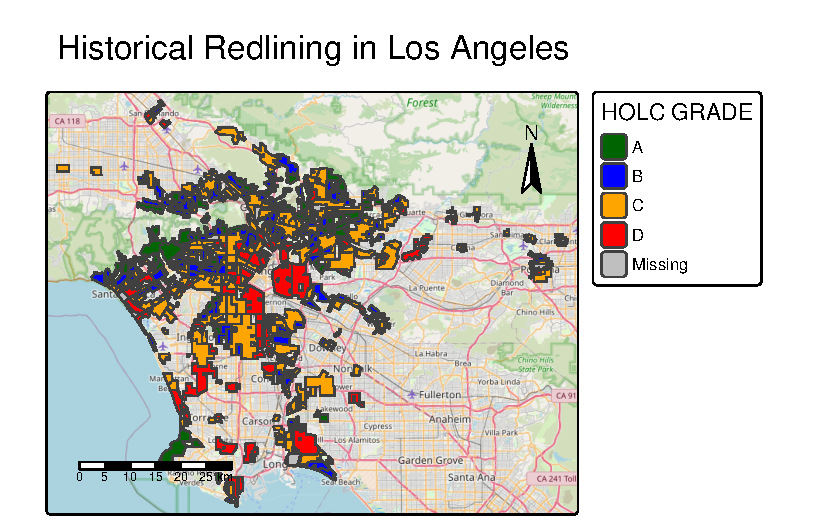
\includegraphics[keepaspectratio]{HW2_files/figure-pdf/unnamed-chunk-6-1.pdf}}

\begin{enumerate}
\def\labelenumi{\arabic{enumi}.}
\setcounter{enumi}{1}
\tightlist
\item
  Spatial join and summary table Assign census block group in ejscreen
  to the HOLC grade it falls inside.
\end{enumerate}

\begin{Shaded}
\begin{Highlighting}[]
\CommentTok{\# Assign HOLC grade to each census block group}

\NormalTok{ej\_holc }\OtherTok{\textless{}{-}} \FunctionTok{st\_join}\NormalTok{(ejscreen, holc[}\StringTok{\textquotesingle{}grade\textquotesingle{}}\NormalTok{])}

\CommentTok{\# Drop geometry for table and statistics}

\NormalTok{ej\_holc\_df }\OtherTok{\textless{}{-}} \FunctionTok{st\_drop\_geometry}\NormalTok{(ej\_holc)}

\CommentTok{\# summary table: \% in each HOLC grade plus \% with no grade}

\NormalTok{grade\_summary }\OtherTok{\textless{}{-}}\NormalTok{ ej\_holc\_df }\SpecialCharTok{\%\textgreater{}\%} 
  \FunctionTok{mutate}\NormalTok{(}\AttributeTok{has\_grade =} \SpecialCharTok{!}\FunctionTok{is.na}\NormalTok{(grade), }\StringTok{"None"}\NormalTok{, grade) }\SpecialCharTok{\%\textgreater{}\%} 
  \FunctionTok{group\_by}\NormalTok{(grade) }\SpecialCharTok{\%\textgreater{}\%} 
  \FunctionTok{summarise}\NormalTok{(}\AttributeTok{n =}\FunctionTok{n}\NormalTok{()) }\SpecialCharTok{\%\textgreater{}\%} 
  \FunctionTok{ungroup}\NormalTok{() }\SpecialCharTok{\%\textgreater{}\%} 
  \FunctionTok{mutate}\NormalTok{(}
    \AttributeTok{pct =}\NormalTok{ n }\SpecialCharTok{/}\FunctionTok{sum}\NormalTok{(n) }\SpecialCharTok{*} \DecValTok{100}
\NormalTok{  )}

\CommentTok{\# Table summary}
\NormalTok{grade\_summary }\SpecialCharTok{\%\textgreater{}\%}  \FunctionTok{gt}\NormalTok{() }\SpecialCharTok{\%\textgreater{}\%}  \FunctionTok{tab\_header}\NormalTok{(}\StringTok{"Percentage of Block Groups by HOLC Grade"}\NormalTok{)}
\end{Highlighting}
\end{Shaded}

\begin{table}
\caption*{
{\fontsize{20}{25}\selectfont  Percentage of Block Groups by HOLC Grade\fontsize{12}{15}\selectfont }
} 
\fontsize{12.0pt}{14.0pt}\selectfont
\begin{tabular*}{\linewidth}{@{\extracolsep{\fill}}lrr}
\toprule
grade & n & pct \\ 
\midrule\addlinespace[2.5pt]
A & 449 & 0.1829532 \\ 
B & 1239 & 0.5048529 \\ 
C & 3058 & 1.2460374 \\ 
D & 1346 & 0.5484520 \\ 
NA & 239326 & 97.5177045 \\ 
\bottomrule
\end{tabular*}
\end{table}

\begin{enumerate}
\def\labelenumi{\arabic{enumi}.}
\setcounter{enumi}{2}
\tightlist
\item
  Summary statistics and visualization summaries
\end{enumerate}

\begin{Shaded}
\begin{Highlighting}[]
\CommentTok{\# Compute means by HOLC grade}
\NormalTok{ej\_mean\_grade }\OtherTok{\textless{}{-}}\NormalTok{ ej\_holc\_df }\SpecialCharTok{\%\textgreater{}\%} 
  \FunctionTok{group\_by}\NormalTok{(grade) }\SpecialCharTok{\%\textgreater{}\%} 
  \FunctionTok{summarise}\NormalTok{(}
    \AttributeTok{mean\_low\_income =} \FunctionTok{mean}\NormalTok{(LOWINCPCT, }\AttributeTok{na.rm =} \ConstantTok{TRUE}\NormalTok{),}
    \AttributeTok{mean\_pm25 =} \FunctionTok{mean}\NormalTok{(P\_PM25, }\AttributeTok{na.rm =} \ConstantTok{TRUE}\NormalTok{),}
    \AttributeTok{mean\_lifeexp =} \FunctionTok{mean}\NormalTok{(LIFEEXPPCT, }\AttributeTok{na.rm =} \ConstantTok{TRUE}\NormalTok{)}
\NormalTok{  ) }\SpecialCharTok{\%\textgreater{}\%} 
  
\CommentTok{\# print(ej\_mean\_grade) checking results}
  
\FunctionTok{pivot\_longer}\NormalTok{(}
    \AttributeTok{cols =} \FunctionTok{c}\NormalTok{(mean\_low\_income, mean\_pm25, mean\_lifeexp),}
    \AttributeTok{names\_to =} \StringTok{"variable"}\NormalTok{,}
    \AttributeTok{values\_to =} \StringTok{"mean\_value"}
\NormalTok{)}


\CommentTok{\# Creating a faceted ggplot}

\FunctionTok{ggplot}\NormalTok{(ej\_mean\_grade, }\FunctionTok{aes}\NormalTok{(}\AttributeTok{x =}\NormalTok{ grade, }\AttributeTok{y =}\NormalTok{ mean\_value, }\AttributeTok{fill =}\NormalTok{ grade)) }\SpecialCharTok{+}
  \FunctionTok{geom\_col}\NormalTok{() }\SpecialCharTok{+}
  \FunctionTok{facet\_wrap}\NormalTok{( }\SpecialCharTok{\textasciitilde{}}\NormalTok{ variable, }\AttributeTok{scales =} \StringTok{\textquotesingle{}free\_y\textquotesingle{}}\NormalTok{) }\SpecialCharTok{+}
  \FunctionTok{labs}\NormalTok{(}
  \AttributeTok{title =} \StringTok{"Mean EJScreen Variables by HOLC Grade"}\NormalTok{,}
  \AttributeTok{x =} \StringTok{"HOLC Grade"}\NormalTok{,}
  \AttributeTok{y =} \StringTok{"Mean Value"}\NormalTok{,}
  \AttributeTok{fill =} \StringTok{"HOLC Grade"}
\NormalTok{  ) }\SpecialCharTok{+}
  \FunctionTok{theme\_minimal}\NormalTok{() }\SpecialCharTok{+}
  \FunctionTok{theme}\NormalTok{(}
    \AttributeTok{strip.text =} \FunctionTok{element\_text}\NormalTok{(}\AttributeTok{size =} \DecValTok{12}\NormalTok{, }\AttributeTok{face =} \StringTok{"bold"}\NormalTok{),}
    \AttributeTok{axis.text.x =} \FunctionTok{element\_text}\NormalTok{(}\AttributeTok{angle =} \DecValTok{0}\NormalTok{, }\AttributeTok{hjust =} \FloatTok{0.5}\NormalTok{),}
    \AttributeTok{plot.title =} \FunctionTok{element\_text}\NormalTok{(}\AttributeTok{size =} \DecValTok{14}\NormalTok{, }\AttributeTok{face =} \StringTok{"bold"}\NormalTok{)}
\NormalTok{  )}
\end{Highlighting}
\end{Shaded}

\pandocbounded{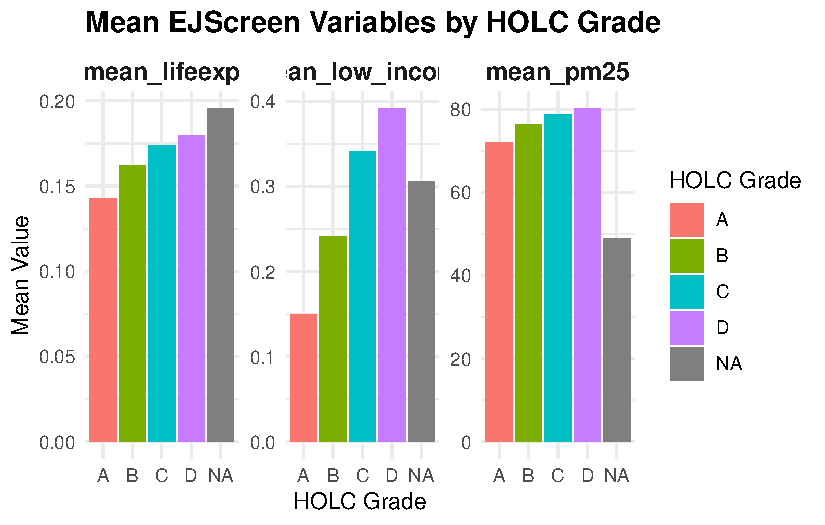
\includegraphics[keepaspectratio]{HW2_files/figure-pdf/unnamed-chunk-8-1.pdf}}

\begin{enumerate}
\def\labelenumi{\arabic{enumi}.}
\setcounter{enumi}{3}
\tightlist
\item
  Reflection paragraph
\end{enumerate}

Historical redlining in Los Angeles show continuous existence
environmental and socioeconomic disparities. Census block groups located
in formerly redlining neighborhoods, HOLC grade D and C, have high
percentages of low\_income residents, elevated particular matter (PM
2.5) exposure, and lower life expectancy percentage compared to areas
with high historical grades (A or B). This pattern suggest that
discrimination continues to shape environmental justice outcomes, while
correlation does not imply causation, these observations align with
literature demonstrating that historic housing redlining influences
inequalities in exposure to pollution and socioeconomic vulnerability.

Part 2: Legacy of redlining in biodiversity observations

Exploring the legacy of historical redlining in Los Angeles on the
collection of bird observations from 2021-2023.

\begin{enumerate}
\def\labelenumi{\arabic{enumi}.}
\tightlist
\item
  Percent observation summary of redlining neighborhoods within each
  HOLC grade.
\end{enumerate}

\begin{Shaded}
\begin{Highlighting}[]
\CommentTok{\# Assigning each bird observation to a HOLC grade}
\NormalTok{birds\_holc }\OtherTok{\textless{}{-}} \FunctionTok{st\_join}\NormalTok{(birds, holc[}\StringTok{"grade"}\NormalTok{])}

\CommentTok{\# Replacing NA grades with "None"}
\NormalTok{birds\_holc }\OtherTok{\textless{}{-}}\NormalTok{  birds\_holc }\SpecialCharTok{\%\textgreater{}\%} 
  \FunctionTok{mutate}\NormalTok{(}\AttributeTok{grades =} \FunctionTok{ifelse}\NormalTok{(}\FunctionTok{is.na}\NormalTok{(grade), }\StringTok{"None"}\NormalTok{, grade))}
\end{Highlighting}
\end{Shaded}

\begin{enumerate}
\def\labelenumi{\arabic{enumi}.}
\setcounter{enumi}{2}
\tightlist
\item
  Bird observation per HOLC grade percent (\%) summery.
\end{enumerate}

\begin{Shaded}
\begin{Highlighting}[]
\NormalTok{bird\_summary }\OtherTok{\textless{}{-}}\NormalTok{ birds\_holc }\SpecialCharTok{\%\textgreater{}\%} 
  \FunctionTok{st\_drop\_geometry}\NormalTok{() }\SpecialCharTok{\%\textgreater{}\%} 
  \FunctionTok{group\_by}\NormalTok{(grade) }\SpecialCharTok{\%\textgreater{}\%} 
  \FunctionTok{summarise}\NormalTok{(}\AttributeTok{n =}\FunctionTok{n}\NormalTok{()) }\SpecialCharTok{\%\textgreater{}\%} 
  \FunctionTok{ungroup}\NormalTok{() }\SpecialCharTok{\%\textgreater{}\%} 
  \FunctionTok{mutate}\NormalTok{(}\AttributeTok{pct =}\NormalTok{ n}\SpecialCharTok{/} \FunctionTok{sum}\NormalTok{(n) }\SpecialCharTok{*} \DecValTok{100}\NormalTok{)}

\FunctionTok{print}\NormalTok{(bird\_summary)}
\end{Highlighting}
\end{Shaded}

\begin{verbatim}
# A tibble: 5 x 3
  grade       n   pct
  <chr>   <int> <dbl>
1 A       30345  2.35
2 B       24198  1.88
3 C       47973  3.72
4 D       30246  2.35
5 <NA>  1156104 89.7 
\end{verbatim}

\begin{enumerate}
\def\labelenumi{\arabic{enumi}.}
\setcounter{enumi}{3}
\tightlist
\item
  Visualization
\end{enumerate}

\begin{Shaded}
\begin{Highlighting}[]
\CommentTok{\# Changing label for NA grades so it doesnt show "NA" in the plot}

\NormalTok{bird\_summary }\OtherTok{\textless{}{-}}\NormalTok{ bird\_summary }\SpecialCharTok{\%\textgreater{}\%} 
  \FunctionTok{mutate}\NormalTok{(}\AttributeTok{grade =} \FunctionTok{ifelse}\NormalTok{(}\FunctionTok{is.na}\NormalTok{(grade), }\StringTok{"Outside HOLC"}\NormalTok{, grade))}

\CommentTok{\# Graph 2.}
\FunctionTok{ggplot}\NormalTok{(bird\_summary, }\FunctionTok{aes}\NormalTok{(}\AttributeTok{x =}\NormalTok{ grade, }\AttributeTok{y =}\NormalTok{ pct, }\AttributeTok{fill =}\NormalTok{ grade)) }\SpecialCharTok{+}
  \FunctionTok{geom\_col}\NormalTok{(}\AttributeTok{show.legend =} \ConstantTok{FALSE}\NormalTok{) }\SpecialCharTok{+}
  \FunctionTok{scale\_y\_continuous}\NormalTok{(}\AttributeTok{labels =}\NormalTok{ scales}\SpecialCharTok{::}\FunctionTok{percent\_format}\NormalTok{(}\AttributeTok{scale =} \DecValTok{1}\NormalTok{)) }\SpecialCharTok{+} \CommentTok{\# format y{-}axis to display \% instead of raw numbers}
   \FunctionTok{scale\_fill\_viridis\_d}\NormalTok{() }\SpecialCharTok{+}
  \FunctionTok{labs}\NormalTok{(}
    \AttributeTok{title =} \StringTok{"Percentage of Birds Observations by HOLC Grade (2021{-}2023)"}\NormalTok{,}
    \AttributeTok{x =} \StringTok{"HOLC Grade"}\NormalTok{,}
    \AttributeTok{y =} \StringTok{"Percent of Observations"}
\NormalTok{  ) }\SpecialCharTok{+}
  \FunctionTok{theme\_minimal}\NormalTok{(}\AttributeTok{base\_size =} \DecValTok{14}\NormalTok{)}
\end{Highlighting}
\end{Shaded}

\pandocbounded{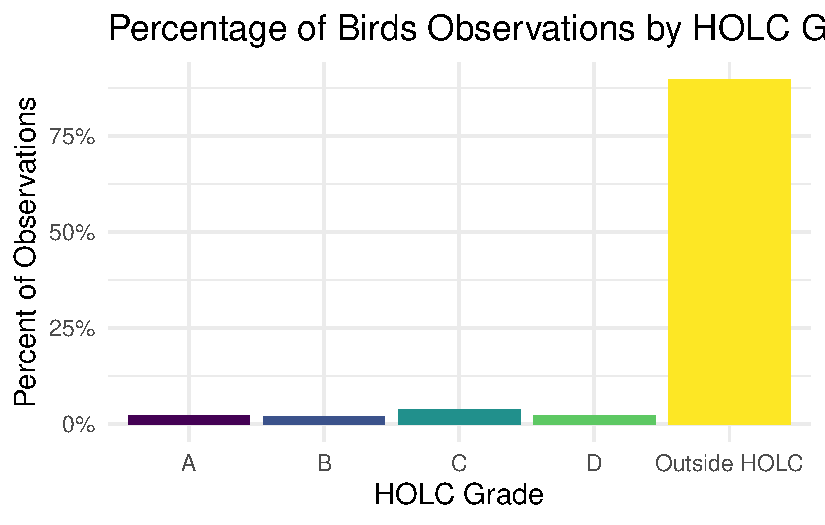
\includegraphics[keepaspectratio]{HW2_files/figure-pdf/unnamed-chunk-11-1.pdf}}

\begin{enumerate}
\def\labelenumi{\arabic{enumi}.}
\setcounter{enumi}{4}
\tightlist
\item
  Reflection
\end{enumerate}

The results show that most bird observations occurred outside
historically redlining areas. Those observation that do fall withing
HOLC graded neighborhoods, Grade C contained the highest share at
3.72\%, following Grade A and D at 2.35 \% each, and Grade B at 1.88\%.
Unlike Ellis-Soto et al.~(2023), we do not observe a clear gradient of
reduced biodiversity observations in formerly redlining areas because
here we only focused on a small geographic scale, LA county while
Ellis\_Soto study accounted for a larger geographic scale, 38 states.




\end{document}
